\documentclass[12pt, titlepage]{article}

\usepackage{booktabs}
\usepackage{tabularx}
\usepackage{hyperref}
\usepackage{graphicx}
\usepackage{subcaption}
\hypersetup{
    colorlinks,
    citecolor=black,
    filecolor=black,
    linkcolor=red,
    urlcolor=blue
}
\usepackage[round]{natbib}

\title{SE 3XA3: Software Requirements Specification\\Red Discord Bot}

\author{Team \#31, R-DB V2
		\\ Jason Tsui tsuij8
		\\ Hareem Arif arifh1
		\\ Abdul Elrahwan elrahwaa
}

\date{\today}


\begin{document}

\maketitle

\pagenumbering{roman}
\tableofcontents
\listoftables
\listoffigures

\begin{table}[!bp]
\caption{\bf Revision History}
\begin{tabularx}{\textwidth}{p{3cm}p{2cm}X}
\toprule {\bf Date} & {\bf Version} & {\bf Notes}\\
\midrule
Oct 4,2018 & 1.0 & Project Drivers, Scope\\
Oct 5,2018 & 1.1 & Added individual use case diagram and function requirements\\
Oct 5, 2018 & 1.1 & Added Requirements, cost, risks, user documentation \\
Oct 16, 2018 & 1.2 & Added more requirements, off-the-shelf solutions, new problems, tasks\\Dec 04, 2018 & 2.0 & Prepared for final submission \\
\bottomrule
\end{tabularx}
\end{table}

\newpage

\pagenumbering{arabic}

This document describes the requirements for software project R-DB V2 for McMaster University 3XA3 FALL 2018.\\

The template for the Software
Requirements Specification (SRS) is a subset of the Volere
template~\citep{RobertsonAndRobertson2012}.



\section{Project Drivers}

\subsection{The Purpose of the Project}
Discord is an application which allows people to host and connect with numerous people into a single community over the internet. In these communities, they are able to communicate with each other by talking or typing in text. Oftentimes these communities grow to have over hundreds of persons and the need for community moderation becomes exponentially difficult. The purpose of R-DB V2, is to provide a means of automating commands to moderate the community, enforce rules, and provide community interaction. 

\subsection{The Stakeholders}

\subsubsection{The Client}
	The client of our product is McMaster University who will be the constantly reviewing R-DB V2 and providing guidance to properly document and redeploy the program.

\subsubsection{The Customers}
	The customers of our product are Discord community moderators and owners. The typical owner and moderator would be persons who oversee a large community with numerous members. It is assumed that owners and moderators are looking to automate certain tasks and provide additional functionalities to their community. 


\subsubsection{Other Stakeholders}
Other stakeholders include Discord inc. who will be providing the framework, environment and API to integrate the R-DB V2 program. They are interested in the success of this project as the bot will provide additional user interface and features to the Discord application.

\subsection{Mandated Constraints}
Description: The product shall run on the Discord applcation API and software\\
Rationale: The product is an additional feature intended for the Discord application\\
Fit criterion: Our bot will be available to all users who use the Discord application\\\\

\noindent
Description: The product shall only operate when connected to the internet\\
Rationale: Discord is an online server voIP and thus the product will also be dependant on internet connection\\
Fit criterion: The product shall only operate if an internet connection is present\\

\subsection{Naming Conventions and Terminology}
\begin{itemize}
\item Bot, Autonomous computer controlled program 
\item VoIP, Acronym which refers to Voice over Internet Protocol. Methodology of communication. 
\item Discord, The VoIP platform that is used for the bot.
\item Host, Store a website or data on a server or other computer so that it can be accessed over the internet.
\item Input, User typed in input into Discord community chat.
\item Song request, to request the bot to play a particular song
\item Moderate, Administrative duties to maintain community rules and integrity
\item Kick, to completely remove a user from a community indefinitely
\item ban, to place restrictions on a user in a community indefinitely 
\item softban, to place a ban for a short time
\item stream, to broadcast realtime
\end{itemize}

\section{Functional Requirements}

\subsection{The Scope of the Work and the Product}

\subsubsection{The Context of the Work}
Project is to produce a Discord bot that is able to automate built-in Discord interfaces and provide additional features. Project is expected to be completed by Winter 2018. The exact details for milestones and goals is under the Development Plan and associated Gantt Chart. 

\subsubsection{Work Partitioning}
Group members are expected to equally contribute. Work tasks will be discussed and partitioned on a meeting-by-meeting basis. Work tasks will be generated on a weekly basis based on goals within the most current Gantt Chart and Development Plan.

\subsubsection{Individual Product Use Cases}
\begin{figure}
   \centering
   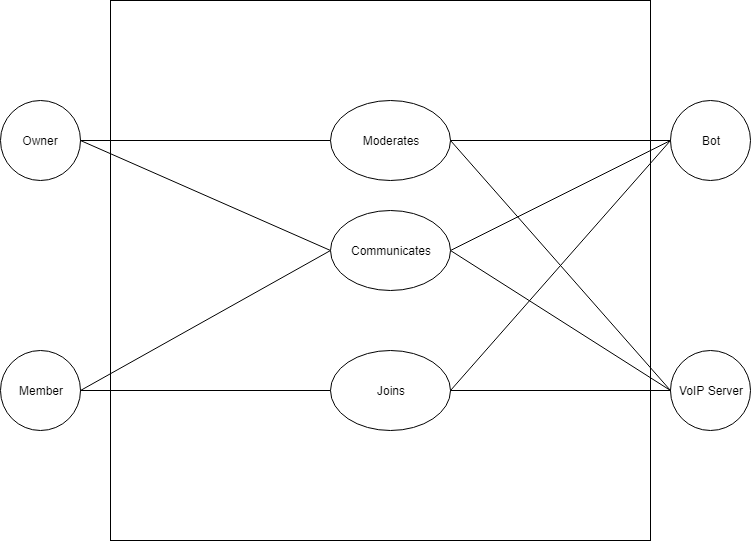
\includegraphics[width=\linewidth]{UseCaseDiagram.png}
   \caption{Use Case Diagram}
  \label{fig:use Case Diagram}
\end{figure}

\subsection{Functional Requirements}
\begin{itemize}
\color{blue}
\item FR1: The bot shall be able to handle music requests from YouTube
\item FR2: The bot shall be able to perform chat cleanup and filtering
\item FR3: The bot shall allow users to search for images on Imgur and send them in the channel
\item FR4: The bot shall create a platform where users earn experience points for participation and level up
\end{itemize}


\section{Non-functional Requirements}

\subsection{Look and Feel Requirements}
Not applicable, since system being built does not have a GUI. 
\subsection{Usability and Humanity Requirements}
\begin{itemize}
\item The software must be simple enough for a person age 12-65 in able condition to use all the features provided and to understand them. 
\color{blue}
\item The user will need to be provided with a list of commands to use
\color{black}
\item There is no crucial error rate that will affect the functionality of the software. 
\item The software will use symbols and words that are understandable to the user community. 
\color{blue}
\item All commands will begin with "!"
\end{itemize}

\subsection{Performance Requirements}
\begin{itemize}
\item Any interaction between the user and the product will have a maximum response time of 5 seconds. 
\item The product will not incur time delays of more than 5 seconds. 
\end{itemize}
\subsection{Operational and Environmental Requirements}
\subsubsection {Expected Physical Environment}
The software is expected to run on any device that Discord is available on.


\subsection{Maintainability and Support Requirements}
\begin{itemize}
\item The source code will be available to the public on GitLab, to open up the room for more people to maintain it.

\item Documentation and comments will be utilized to help programmers understand how the source code work and make it easier for them to add new functionalities for the software.
\end{itemize}
\subsection{Security Requirements}
\begin{itemize}
\item The software must be protected from unauthorized attempts to read and/manipulate the user’s data
\item The software must not be withholding any data the user did not consent to release.
\end{itemize}

\subsection{Cultural Requirements}
\begin{itemize}
\item The product will not utilize any content (images, text, video, other media) that is considered offensive.
\item The product will not be offensive to any ethnic groups
\item The product will not be offensive to any religious groups
\color{blue}
\item The cultural requirements will be upheld by Imgur and Youtube's own community standards policies
\end{itemize}
\subsection{Legal Requirements}
\begin{itemize}
\item The software will comply with all details entailed with regards to licensing 
\item All copyright conditions and obligations enforced by law will be met 
\end{itemize}
\subsection{Health and Safety Requirements}
\color{blue} Not available
\color{black}

\section{Project Issues}

\subsection{Open Issues}
\begin{itemize}
\color{blue}
\item Images modules needs to let users see the image before sending it
\color{black}
\end{itemize}

\subsection{Off-the-Shelf Solutions}

There are many publicly available Discord  bots with many similar functionalities to the product we are creating. Similar bots include MiBro, AnthBot, and The Bastion Bot. Many of the aforementioned bots contain components that would be helpful to study for our implementation.

\subsection{New Problems}
A potential problem would be people using the bot to spam the chat. Taken into consideration that the bot displays images and plays music, some users can use those features to spam the chat.

\subsection{Tasks}
The tasks for this project must follow the deliverables for Software Engineering 3xa3. Additional tasks were decided on by the group members. 

\subsection{Migration to the New Product}

\subsection{Risks}

\begin{itemize}
\item Excessive schedule pressure – due to reimplementation of various aspects of the product that are of significant value.
\end{itemize}

\subsection{Costs}

No additional cost will be incurred by the developers nor the users to use the product and all the offered features. 

\subsection{User Documentation and Training}

User will be provided with introductory documentation to explain the operability of the software to get user started, no additional training will be required. 

\subsection{Waiting Room}

NA

\subsection{Ideas for Solutions}

\bibliographystyle{plainnat}

\bibliography{SRS}

\newpage

\section{Appendix}

This section has been added to the Volere template.  This is where you can place
additional information.

\subsection{Symbolic Parameters}

The definition of the requirements will likely call for SYMBOLIC\_CONSTANTS.
Their values are defined in this section for easy maintenance.

NA 

\end{document}